\tikzset{
   plane/.pic = {
    \draw[fill]  plot[smooth, tension=0.6] coordinates {
        (-0.65,-0.9) 
        (-0.6,-0.85) 
        (-0.4,-0.75) 
        (-0.25,-0.65) 
        (-0.15,-0.5) 
        (-0.12,-0.3) 
        (-0.1,-0.1) 
        (0,0) 
        (0.1,-0.1) 
        (0.12,-0.3) 
        (0.15,-0.5) 
        (0.25,-0.65) 
        (0.4,-0.75) 
        (0.6,-0.85) 
        (0.65,-0.9)
        } -- plot[smooth, tension=0.6] coordinates {
        (0.65,-0.9) 
        (0.15,-0.91)
        (0.35,-1.1) 
        (0.37,-1.15)
        } -- plot[smooth, tension=0.6] coordinates {
        (0.37,-1.15)
        (0,-1.12) 
        (-0.37,-1.15) 
        } -- plot[smooth, tension=0.6] coordinates {
        (-0.37,-1.15)
        (-0.35,-1.1) 
        (-0.15,-0.91) 
        (-0.65,-0.9) 
        } -- cycle;
   }
}

\usetikzlibrary{math}

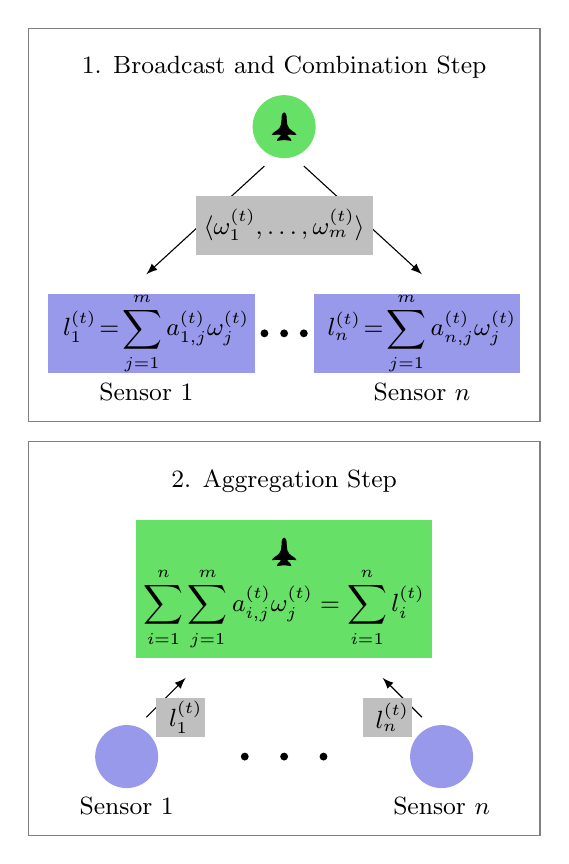
\begin{tikzpicture}[font=\small]
    % Step 1
    \node at (3.25,5.5) {1. Broadcast and Combination Step};
    % Navigator
    \fill (3.25,4.75) [green!80!black!60] ellipse (0.4 and 0.4);
    \pic[xscale=0.22,yscale=0.3] at (3.25,4.9225) {plane};
    % Sensors
    \node at (1.5,1.375) {Sensor $1$};
    \fill [blue!80!black!40] (0.25,1.625) rectangle (2.875,2.625);
    \node at (1.625,2.125) {$\displaystyle l_1^{(t)} \!=\! \sum^m_{j=1}a_{1,j}^{(t)}\omega_j^{(t)}$};
    \node at (5,1.375) {Sensor $n$};
    \fill [blue!80!black!40] (3.625,1.625) rectangle (6.25,2.625);
    \node at (5,2.125) {$\displaystyle l_n^{(t)} \!=\! \sum^m_{j=1}a_{n,j}^{(t)}\omega_j^{(t)}$};
    \fill [black] (3.5,2.125) circle (0.05);
    \fill [black] (3,2.125) circle (0.05);
    \fill [black] (3.25,2.125) circle (0.05);
    % Lines
    \draw [-latex] plot[smooth, tension=.7] coordinates {(3.5,4.25) (5,2.875)};
    \draw [-latex] plot[smooth, tension=.7] coordinates {(3,4.25) (1.5,2.875)};
    \fill [lightgray] (2.125,3.875) rectangle (4.375,3.125);
    \node at (3.25,3.5) {$\langle\omega_1^{(t)},\dots ,\omega_m^{(t)}\rangle$};
    
    % Step 2
    \node at (3.25,0.25) {2. Aggregation Step};
    % Navigator
    \fill [green!80!black!60] (1.375,-2) rectangle (5.125,-0.25);
    \pic[xscale=0.22,yscale=0.3] at (3.25,-0.4775) {plane};
    \node at (3.25,-1.375) {$\displaystyle \sum^{n}_{i=1}\sum^{m}_{j=1} a_{i,j}^{(t)}\omega_j^{(t)} = \sum^n_{i=1}l^{(t)}_{i}$};
    % Sensors
    \node at (1.25,-3.875) {Sensor $1$};
    \fill  (5.25,-3.25) [blue!80!black!40] ellipse (0.4 and 0.4);
    \node at (5.25,-3.875) {Sensor $n$};
    \fill  (1.25,-3.25) [blue!80!black!40] ellipse (0.4 and 0.4);
    \fill [black] (2.75,-3.25) circle (0.05);
    \fill [black] (3.75,-3.25) circle (0.05);
    \fill [black] (3.25,-3.25) circle (0.05);
    % Lines
    \draw [-latex] plot[smooth, tension=.7] coordinates {(5,-2.75) (4.5,-2.25)};
    \draw [-latex] plot[smooth, tension=.7] coordinates {(1.5,-2.75) (2,-2.25)};
    \fill [lightgray] (1.625,-2.5) rectangle (2.25,-3);
    \node at (2,-2.75) {$l_1^{(t)}$};
    \fill [lightgray] (4.25,-2.5) rectangle (4.875,-3);
    \node at (4.625,-2.75) {$l_n^{(t)}$};
    
    % Bounding rectangles
    \draw [gray] (0,6) rectangle (6.5,1);
    \draw [gray] (0,0.75) rectangle (6.5,-4.25);
\end{tikzpicture}